%% Le lingue utilizzate, che verranno passate come opzioni al pacchetto babel. Come sempre, l'ultima indicata sarà quella primaria.
%% Se si utilizzano una o più lingue diverse da "italian" o "english", leggere le istruzioni in fondo.
\def\thudbabelopt{english,italian}
%% Valori ammessi per target: bach (tesi triennale), mst (tesi magistrale), phd (tesi di dottorato).
%% Valori ammessi per aauheader: '' (vuoto -> nessun header Alpen Adria Univeristat), aics (Department of Artificial Intelligence and Cybersecurity), informatics (Department of Informatics Systems). Il nome del dipartimento è allineato con la versione inglese del logo UniUD.
%% Valori ammessi per style: '' (vuoto -> stile moderno), old (stile tradizionale).
\documentclass[target=bach,aauheader=,style=]{thud}

%% --- Informazioni sulla tesi ---
%% Per tutti i tipi di tesi
% Scommentare quello di interesse, o mettete quello che vi pare
\course{Informatica}
%\course{Internet of Things, Big Data e Web}
%\course{Matematica}
%\course{Comunicazione Multimediale e Tecnologie dell'Informazione}
\title{Un sistema distribuito per l'analisi della topologia di reti di calcolatori}
\author{Diego Cirillo}
\supervisor{Prof.\ Marino Miculan}
\cosupervisor{Dott.\ Matteo Paier}
%\tutor{Guido Necchi}
%% Campi obbligatori: \title, \author e \course.
%% Altri campi disponibili: \reviewer, \tutor, \chair, \date (anno accademico, calcolato in automatico), \rights
%% Con \supervisor, \cosupervisor, \reviewer e \tutor si possono indicare più nomi separati da \and.
%% Per le sole tesi di dottorato:
%\phdnumber{313}
%\cycle{XXVIII}
%\contacts{Via della Sintassi Astratta, 0/1\\65536 Gigatera --- Italia\\+39 0123 456789\\\texttt{http://www.example.com}\\\texttt{inbox@example.com}}

%% --- Pacchetti consigliati ---
%% pdfx: per generare il PDF/A per l'archiviazione. Necessario solo per la versione finale
\usepackage[a-1b]{pdfx}
%% hyperref: Regola le impostazioni della creazione del PDF... più tante altre cose. Ricordarsi di usare l'opzione pdfa.
\usepackage[pdfa]{hyperref}
%% tocbibind: Inserisce nell'indice anche la lista delle figure, la bibliografia, ecc.
\graphicspath{ {./images/} }
%% --- Stili di pagina disponibili (comando \pagestyle) ---
%% sfbig (predefinito): Apertura delle parti e dei capitoli col numero grande; titoli delle parti e dei capitoli e intestazioni di pagina in sans serif.
%% big: Come "sfbig", solo serif.
%% plain: Apertura delle parti e dei capitoli tradizionali di LaTeX; intestazioni di pagina come "big".

\begin{document}
\maketitle

%% Dedica (opzionale)
%\begin{dedication}
%	Al mio cane,\par per avermi ascoltato mentre ripassavo le lezioni.
%\end{dedication}

%% Ringraziamenti (opzionali)
%\acknowledgements
%Sed vel lorem a arcu faucibus aliquet eu semper tortor. Aliquam dolor lacus, semper vitae ligula sed, blandit iaculis leo. Nam pharetra lobortis leo nec auctor. Pellentesque habitant morbi tristique senectus et netus et malesuada fames ac turpis egestas. Fusce ac risus pulvinar, congue eros non, interdum metus. Mauris tincidunt neque et aliquam imperdiet. Aenean ac tellus id nibh pellentesque pulvinar ut eu lacus. Proin tempor facilisis tortor, et hendrerit purus commodo laoreet. Quisque sed augue id ligula consectetur adipiscing. Vestibulum libero metus, lacinia ac vestibulum eu, varius non arcu. Nam et gravida velit.

%% Sommario (opzionale)
\abstract
Nunc ac dignissim ipsum, quis pulvinar elit. Mauris congue nec leo ornare lobortis. Nulla hendrerit pretium diam nec lobortis. Nullam aliquam laoreet nisl, sit amet facilisis lectus accumsan ut. Duis et elit hendrerit metus venenatis condimentum. Integer id eros molestie, interdum leo sit amet, aliquet metus. Integer fermentum tristique magna, vel luctus neque rhoncus vel. Ut hendrerit et quam et semper. Mauris egestas, odio sed aliquet luctus, magna orci euismod odio, vitae lacinia tellus tellus non lectus. Aliquam urna neque, porta et mattis aliquam, congue sit amet lorem. In ultrices augue sit amet ante vehicula, vitae rhoncus turpis auctor. Donec porta scelerisque eros, at mollis enim imperdiet ut. 

%% Indice
\tableofcontents

%% Lista delle tabelle (se presenti)
%\listoftables

%% Lista delle figure (se presenti)
%\listoffigures

%% Corpo principale del documento
\mainmatter

%% Parte
%% La suddivisione in parti è opzionale; solitamente sono sufficienti i capitoli.
%\part{Parte}

%% Capitolo
\chapter{Introduzione}
In hac habitasse platea dictumst. Vestibulum consectetur dictum pellentesque. Suspendisse nunc neque, commodo ac imperdiet nec, sollicitudin vitae libero. Donec bibendum vel nunc vitae pharetra. In vel volutpat odio, et interdum dui. Duis mauris ligula, congue eget molestie at, tincidunt nec diam. Nam vitae eros nec arcu suscipit vehicula. Aliquam consectetur imperdiet elit, eget pretium arcu fringilla at. Maecenas \cite{Knu86} sed libero pulvinar, mattis tortor vel, fermentum enim.

%% Sezione
\section{Titolo della Sezione}
Donec pulvinar neque non lectus vulputate pellentesque. Quisque rutrum arcu velit, in feugiat sapien posuere vel. Praesent metus orci, aliquam ac cursus eget, fermentum a nisl. Etiam eu augue lacus. Nam nisi sapien, mattis sed vehicula non, pellentesque at quam. Sed euismod, dolor nec commodo lobortis, erat erat ultricies eros, bibendum dictum nulla felis in dui. Nulla blandit ultrices arcu, vitae lacinia tellus tempor sit amet. Nulla non tincidunt dolor. In eget luctus sem, sed elementum ligula. Proin elementum adipiscing sem, sit amet ultricies nisl tincidunt eu. Ut lobortis dui quam, et scelerisque erat ultrices sit amet. Sed libero sem, mollis quis euismod quis, suscipit ac justo.

%% Sottosezione
\subsection{Sottosezione}
Donec cursus tortor eget sem ornare imperdiet. Ut vel orci non ipsum condimentum laoreet vitae ut sapien. Aenean metus mi, vehicula quis turpis nec, porttitor blandit dui. Nullam sed sollicitudin quam. Fusce nisl ante, commodo eget lacus ac, mollis ullamcorper neque. Quisque faucibus dictum nisl, dignissim fermentum sapien fringilla vel. Proin dui velit, molestie sit amet sapien et, pellentesque tristique purus. Curabitur ac quam ac diam varius bibendum.


%% Capitolo
\chapter{Stato dell'arte}
\label{art}
\section{Premessa}
Questo capitolo è dedicato alla specificazione della architettura generale del sistema prima delle modifiche 

\section{Architettura}
Il sistema è composto da una architettura client-server nella quale il backend si occupa di fare le scansioni e di salvarne i risultati e di fornirli al frontend dove possono essere visualizzati dagli utenti dovrebbero interagire solo con esso. 

\begin{figure}[h]
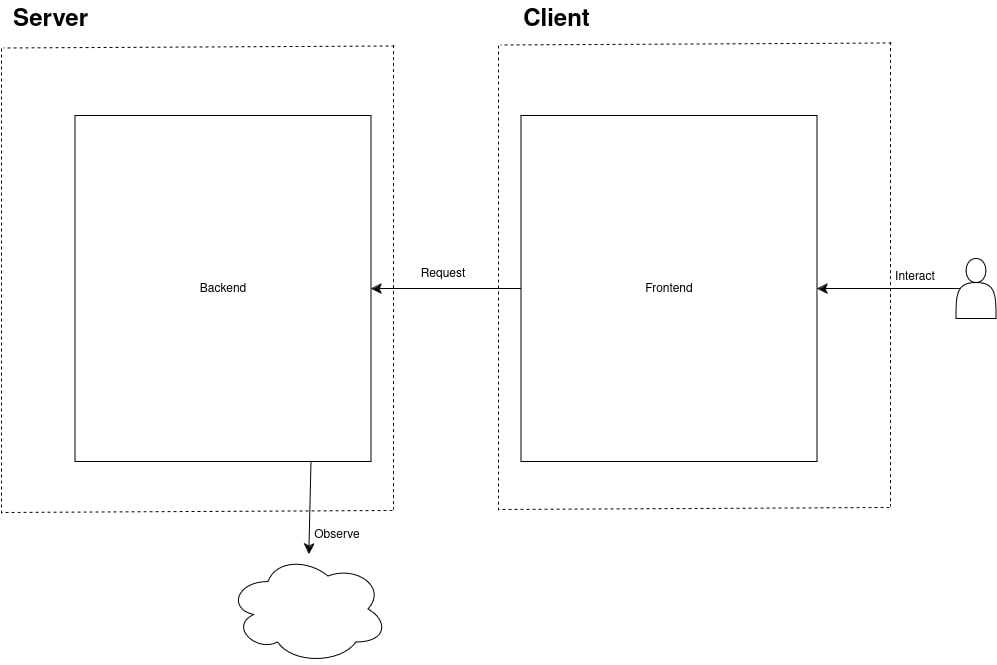
\includegraphics[width=15cm, height=10cm]{client_server}
\centering
\end{figure}

Per organizzazione e scalabilità abbiamo diviso l'architettura in 6 moduli principali.

\begin{figure}[h]
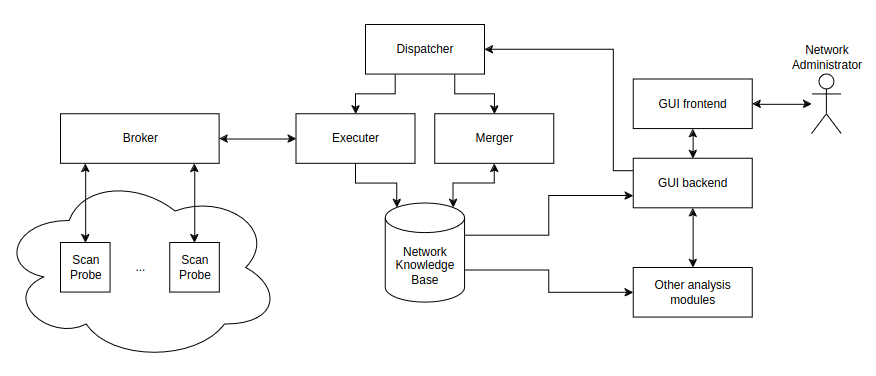
\includegraphics[width=15cm, height=10cm]{moduli_new}
\centering
\end{figure}

\subsection{Scan Probes}
\textbf{Scan Probes} sono moduli che vengono collocati in giro per la rete a raccogliere informazoini. 
Ricevuto un comando il probe lo interpreta, esegue l'opportuna scansione e deserializza il 'output dello scan.

\begin{figure}[h]
  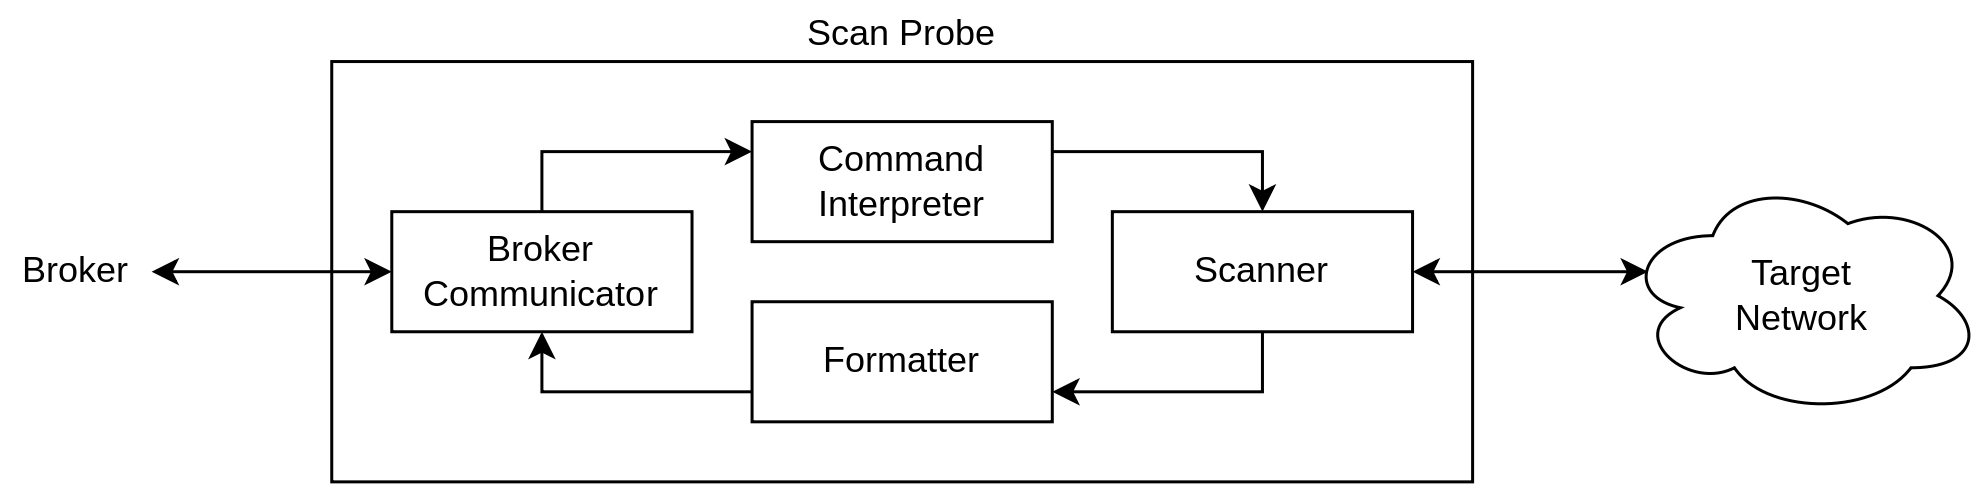
\includegraphics[width=15cm, height=10cm]{probe}
\centering
\end{figure}

\subsection{Dispatcher} 
Il \textbf{Dispatcher} è il modulo che controlla e coordina le operazioni necessarie per le esecuzioni delle scansioni.
Riceve un comando dal Frontend che viene interpretato e mandato allo Scheduler che interagisce con l'Executer ed il Merger per eseguire la scansione e salvarla.

\begin{figure}[h]
  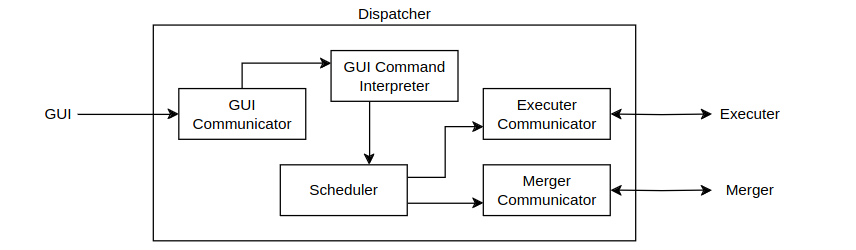
\includegraphics[width=15cm, height=10cm]{dispatcher}
\centering
\end{figure}


\subsection{Executer} 
L'\textbf{Executer} riceve un comando dallo scheduler e coordina gli Scan Probes nell'esecuzione della scansione per poi accumulare i loro risultati e mandarli al Knowledge Base Connector.

\begin{figure}[h]
  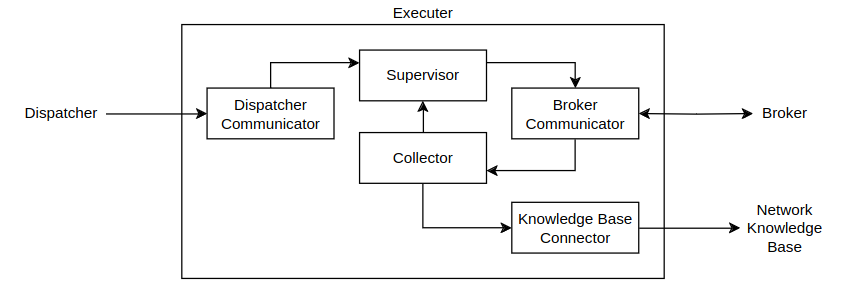
\includegraphics[width=15cm, height=10cm]{executer}
\centering
\end{figure}

\subsection{Merger}
Il \textbf{Merger} si occupa di ricevere i dati generati dai Scan Probes ed amalgamarli per creare un'immagine comprensibile della rete analizzata. 


\begin{figure}[h]
  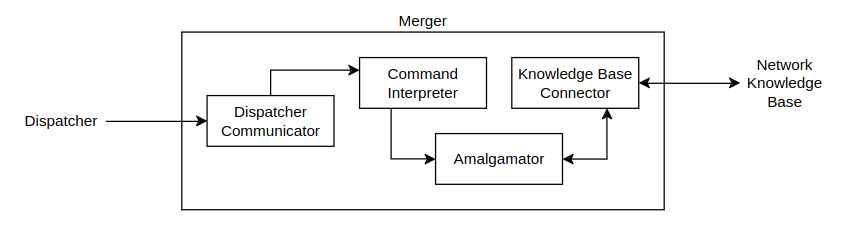
\includegraphics[width=15cm, height=10cm]{merger}
\centering
\end{figure}


\section{programmi}

\subsection{Communication Backbone}
Per comunicare con i probes situati per la rete viene usato MQTT (Message Queuing Telemtry Transport). 
MQTT è un protocollo di messaggistica leggero e public/subscribe progettato per l'Internet of Things (IoT).
Come broker MQTT viene usato Mosquitto per il suo supporto al Qualify of Service livello 2 che garantisce la recezione di messaggi exactly-once fra i probes e il sistema.

\subsection{Scanner}
I probe per eseguire le analisi usano NMAP che è una utility gratis ed open source per fare network discovery anche usata da moltissimi amministratori di reti per fare inventari di rete e monitorare host e servizi. 

\subsection{Tauri}
Il framework Tauri offre la creazione di interfacce moderne, intuitive e sicure.
Per il frontend abbiamo scelto di usare principalmente React; una libreria di TypeScript  open-source sviluppata per la creazione di interfacce utente dinamiche e performanti tramite la costruzioni di UI complesse scomponibili in componenti riutilizzabili.
Il frontend è soprattutto scritto in Rust; un linguaggio di programmazione moderno, compilato e multi-paradigma. Nato con l'obiettivo di coniugare efficienza, sicurezza e affidabilità.


\section{Moduli}
Il frontend è diviso in due moduli che permettono all'utente di interagire con il backend che a sua volta è composto da 5 moduli. 

I due moduli del frontend sono:
\begin{itemize}
  \item L' \textbf{interfaccia web} che l'utente usa per interagire con il sistema. 
  \item Un \textbf{binario eseguibile} che rende possibile l'interazione tra il backend ed l'interfaccia
\end{itemize}

Mentre i cinque moduli del backend:
\begin{itemize}
  \item Il \textbf{Server} che implementa un servizio REST, ovvero un interfaccia che può venir usata per lo scambio di informazioni tra 2 computer.
  \item Lo \textbf{Scheduler} che aspetta per le nuove richieste di scansione e coordina appositamente lo \textit{Scanner} ed il \textit{Parser}.
  \item Lo \textbf{Scanner} riceve la richieste dallo \textit{Scheduler} ed esegue la scansione di \textit{NMAP}.
  \item Il \textbf{Parser} riceve i dati dallo \textit{Scanner} e li processa in modo adeguato.
  \item Lo \textbf{Storage} infine salva e rende a disposizione i dati processati dal \textit{Parser} in un'apposito archivio.
\end{itemize}

\begin{figure}[h]
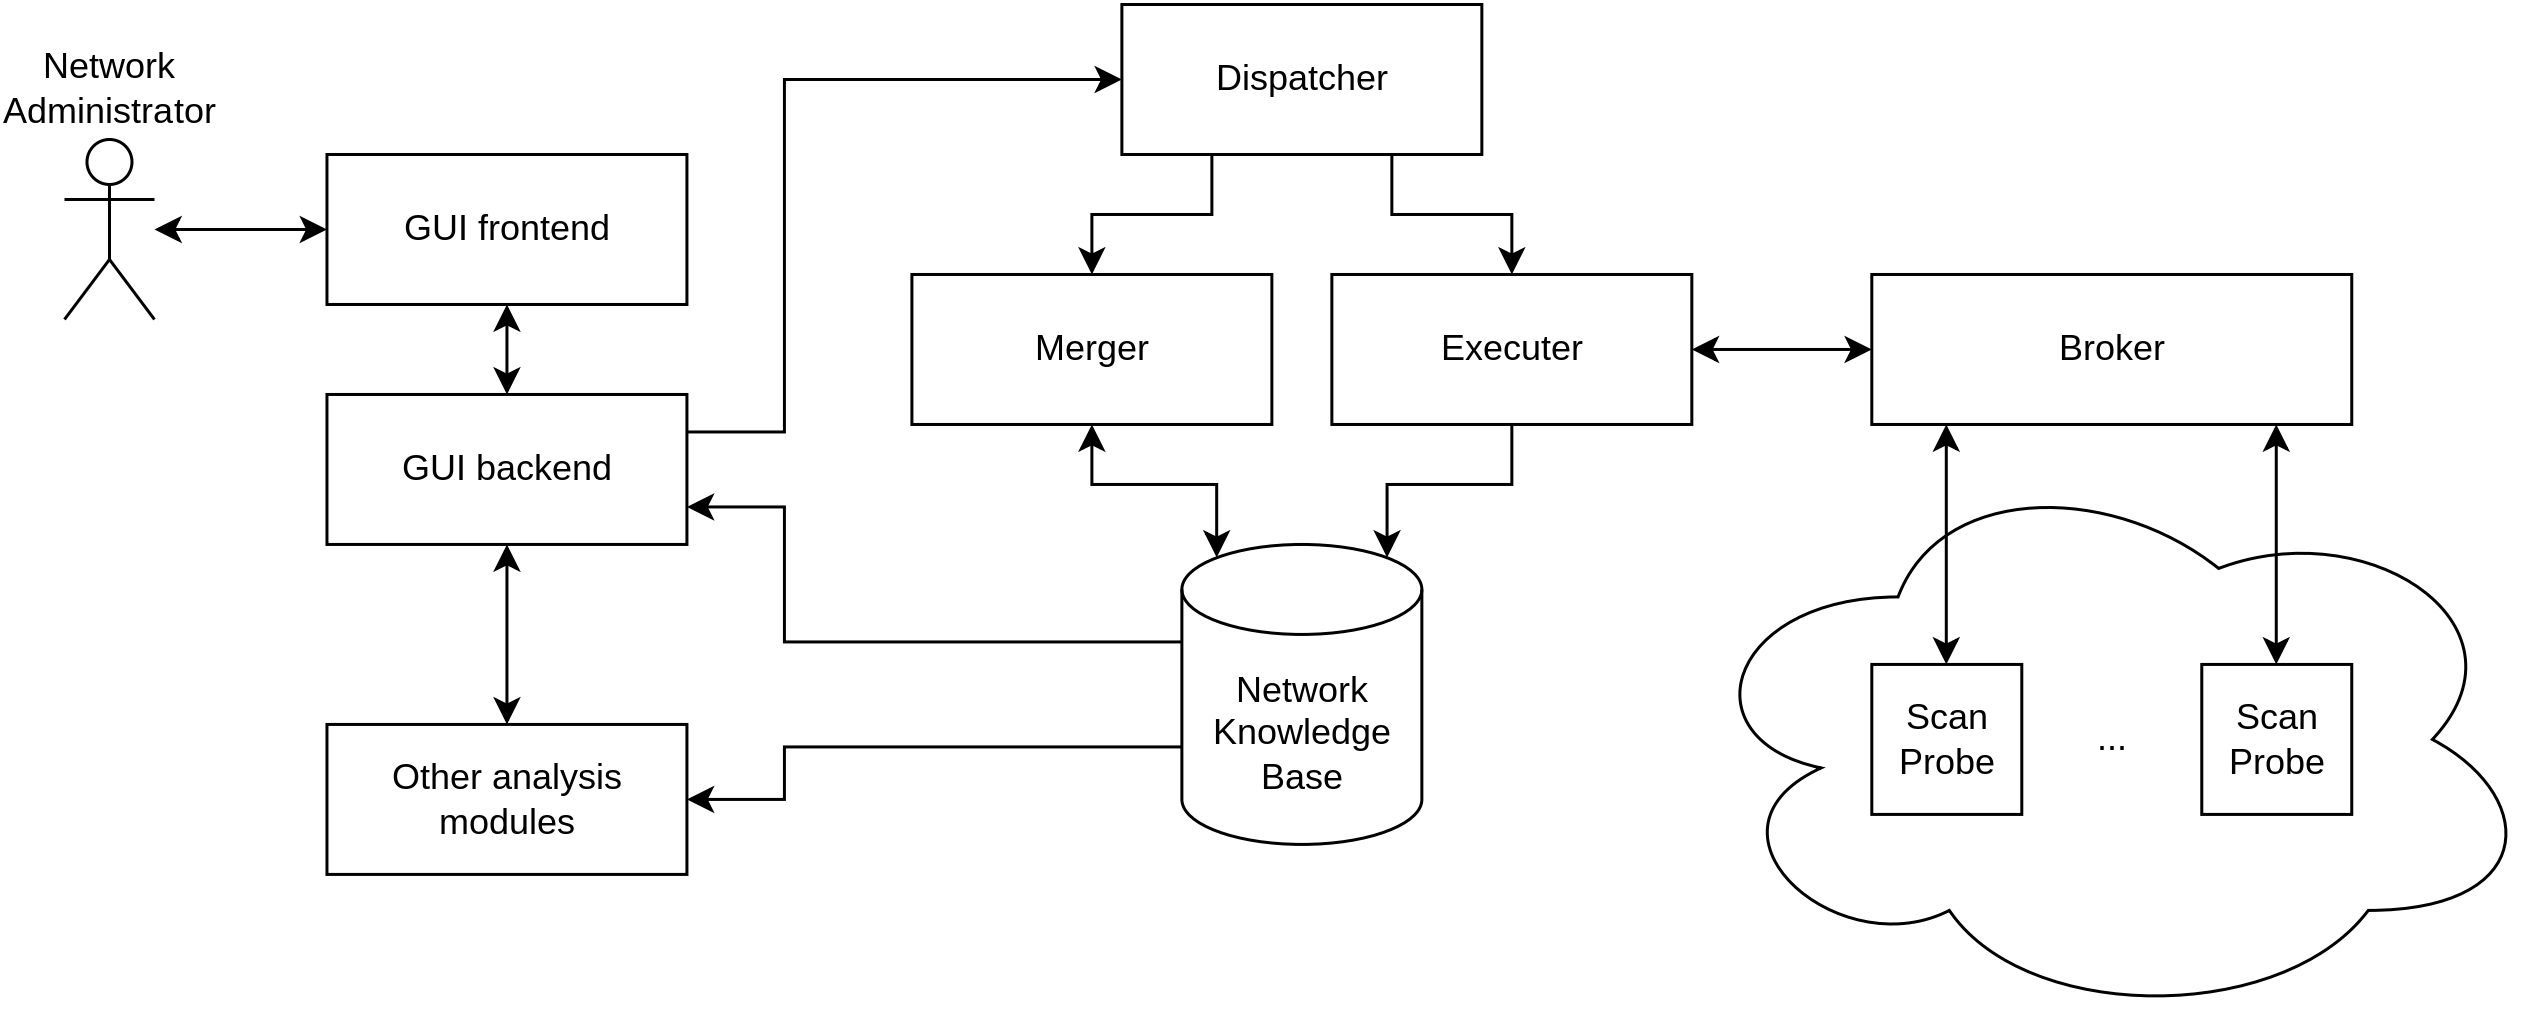
\includegraphics[width=15cm, height=10cm]{moduli}
\centering
\end{figure}

\section{Server}
Il \textbf{Server} è il componente che si comporta da web server e che da a disposizione gli endpoints dell'API usata per la comunicazione tra i vari moduli.

\section{Scanner}
Lo \textbf{Scanner} è il modulo che fa partire la scansione di \textbf{NMAP} quando viene richiesta dallo scheduler. 
NMAP è una utility gratis ed open source per fare network discovery anche usata da moltissimi amministratori di reti per fare inventari di rete e monitorare host e servizi. 
Oltre ad essere popolare e molto potente è anche ben documentata, flessibile e supportata.

\section{Scheduler}
Lo \textbf{Scheduler} è implementato con un piccolo servizio web che ascolta per richieste POST dal frontend(utente) per poi inviare una richiesta json contentente i parametri di scansione allo scanner.

\section{Parser}
Il \textbf{Parser} dopo aver ricevuto in input dallo Scanner un documento \textbf{XML} creato da NMAP inizia un processo di deserializzazione in un oggetto capibile dal programma che poi verrà inserito nello storage.

\section{Storage}
Lo \textbf{Storage} viene gestito da un programma esterno chiamiato \textbf{MongoDB}. 
MongoDB è un database \textbf{NoSQL} con scalabilità e flessibilità che salva i dati in documenti JSON-like facili da gestire.

\section{Linguaggi di programmazione}
Per il backend viene utilizzato Rust mentre per il frontend TypeScript. 
\subsection{Rust}
Rust è un linguaggio di programmazione moderno, compliato e multi-paradigma, sviluppato da Mozilla Research in collaborazoine con la comunità open-source. Nato con l'obiettivo di coniugare efficienza, sicurezza e affidabilità, Rust si distingue per le sue caratteristiche peculiari:
\begin{itemize}
  \item \textbf{Sicurezza della memoria}: Rust elimina la possibilità di dangling pointers e memory leaks, tipici problemi di altri linguaggi che causano crash e comportamenti inaspettati.
  \item \textbf{Prestazioni elevate}: Rust offre prestazioni paragonabili a quelle del C++, grazie alla compilazione in codice macchina efficiente e all'assenza di runtime overhead.
  \item \textbf{Concorrenza sicura}: Rust gestisce la concorrenza in modo nativo, prevenendo automaticamente i data race e garantendo la sicurezza dei thread senza la necessità di complessi meccanismi di sincronizzazione.
  \item \textbf{Produttività}: Rust offre un sistema di ownership moderno e un potente sistema di tipi che aiutano a scrivere codice pulito, conciso e robusto.
\end{itemize}

\subsection{TypeScript}
TypeScript è un superset di JavaScript, ovvero un linguaggio che estende le sue funzionalità con tipi statici, classi, interfacce e moduli opzionali. È stato sviluppato da Microsoft e rilasciato nel 2012, guadagnando rapidamente popolarità nella community di sviluppo web.
Dei punti chiave di TypeScript sono:

\begin{itemize}
  \item \textbf{Tipizzazione statica}: TypeScript consente di definire i tipi di dati per variabili e funzioni, migliorando la leggibilità, la manutenibilità e la robustezza del codice. Il compilatore di TypeScript verifica che i tipi vengano utilizzati correttamente, aiutando a prevenire errori durante l'esecuzione.
  \item \textbf{Maggiori funzionalità}: TypeScript introduce concetti come classi, interfacce e moduli, che facilitano la scrittura di codice strutturato, modulare e scalabile. Queste funzionalità sono particolarmente utili per progetti di grandi dimensioni.
  \item \textbf{Compilazione in JavaScript}: Il codice TypeScript viene compilato in JavaScript puro, che può essere eseguito da qualsiasi browser o motore JavaScript. Questo significa che è possibile utilizzare TypeScript per sviluppare applicazioni web moderne senza preoccuparsi della compatibilità.
\end{itemize}


\section{Frameworks e librerie}
\subsection{Rust}
Le librerie principali usate in Rust sono:
\begin{itemize}
  \item \textbf{Serde}: un framwork per la serializzazione e la deserializzazione per Rust, che consente di convertire facilmente dati strutturati in formati binari come JSON, BSON, XML ed altri. 
  \item \textbf{Tokio}: un runtime asincrono per Rust. Fornisce i mattoni essenziali per la scrittura di applicazioni di rete offrendo elevata velocità, scalabilità, facilità d'uso, affidabilità, robustezza e flessibilità.
  \item \textbf{Tracing} è uno strumento prezioso per la risoluzione dei problemi, il debug e il monitoraggio delle prestazioni di applicazioni Rust complesse.
\end{itemize}

\subsection{TypeScript}
La libreria principale per l'interfaccia grafica è React, una libreria open-source sviluppata da Meta per la creazoine di interfacce utente dinamiche e perfomanti. 
Permette di costruire UI complesse scomponendole in componenti riutilizzabili, facilidando lo sviluppo e la manutenzoine di applicazioni web.

%% Capitolo
\chapter{Lavoro principale}
In hac habitasse platea dictumst. Vestibulum consectetur dictum pellentesque. Suspendisse nunc neque, commodo ac imperdiet nec, sollicitudin vitae libero. Donec bibendum vel nunc vitae pharetra. In vel volutpat odio, et interdum dui. Duis mauris ligula, congue eget molestie at, tincidunt nec diam. Nam vitae eros nec arcu suscipit vehicula. Aliquam consectetur imperdiet elit, eget pretium arcu fringilla at. Maecenas \cite{Knu86} sed libero pulvinar, mattis tortor vel, fermentum enim.


%% Capitolo
\chapter{Risultati}
In hac habitasse platea dictumst. Vestibulum consectetur dictum pellentesque. Suspendisse nunc neque, commodo ac imperdiet nec, sollicitudin vitae libero. Donec bibendum vel nunc vitae pharetra. In vel volutpat odio, et interdum dui. Duis mauris ligula, congue eget molestie at, tincidunt nec diam. Nam vitae eros nec arcu suscipit vehicula. Aliquam consectetur imperdiet elit, eget pretium arcu fringilla at. Maecenas \cite{Knu86} sed libero pulvinar, mattis tortor vel, fermentum enim.


%% Capitolo
\chapter{Conclusioni}
In hac habitasse platea dictumst. Vestibulum consectetur dictum pellentesque. Suspendisse nunc neque, commodo ac imperdiet nec, sollicitudin vitae libero. Donec bibendum vel nunc vitae pharetra. In vel volutpat odio, et interdum dui. Duis mauris ligula, congue eget molestie at, tincidunt nec diam. Nam vitae eros nec arcu suscipit vehicula. Aliquam consectetur imperdiet elit, eget pretium arcu fringilla at. Maecenas \cite{Knu86} sed libero pulvinar, mattis tortor vel, fermentum enim.

%% Fine dei capitoli normali, inizio dei capitoli-appendice (opzionali)
\appendix

%\part{Appendici}

\chapter{Titolo della prima appendice}
Sed purus libero, vestibulum ut nibh vitae, mollis ultricies augue. Pellentesque velit libero, tempor sed pulvinar non, fermentum eu leo. Duis posuere eleifend nulla eget sagittis. Nam laoreet accumsan rutrum. Interdum et malesuada fames ac ante ipsum primis in faucibus. Curabitur eget libero quis leo porttitor vehicula eget nec odio. Proin euismod interdum ligula non ultricies. Maecenas sit amet accumsan sapien.

%% Parte conclusiva del documento; tipicamente per riassunto, bibliografia e/o indice analitico.
\backmatter

%% Riassunto (opzionale)
%\summary
%Maecenas tempor elit sed arcu commodo, dapibus sagittis leo egestas. Praesent at ultrices urna. Integer et nibh in augue mollis facilisis sit amet eget magna. Fusce at porttitor sapien. Phasellus imperdiet, felis et molestie vulputate, mauris sapien tincidunt justo, in lacinia velit nisi nec ipsum. Duis elementum pharetra lorem, ut pellentesque nulla congue et. Sed eu venenatis tellus, pharetra cursus felis. Sed et luctus nunc. Aenean commodo, neque a aliquam bibendum, mauris augue fringilla justo, et scelerisque odio mi sit amet diam. Nulla at placerat nibh, nec rutrum urna. Donec ut egestas magna. Aliquam erat volutpat. Phasellus vestibulum justo sed purus mattis, vitae lacinia magna viverra. Nulla rutrum diam dui, vel semper mi mattis ac. Vestibulum ante ipsum primis in faucibus orci luctus et ultrices posuere cubilia Curae; Donec id vestibulum lectus, eget tristique est.

%% Bibliografia (praticamente obbligatoria)
\bibliographystyle{plain_\languagename}%% Carica l'omonimo file .bst, dove \languagename è la lingua attiva.
%% Nel caso in cui si usi un file .bib (consigliato)
\bibliography{thud}
%% Nel caso di bibliografia manuale, usare l'environment thebibliography.

%% Per l'indice analitico, usare il pacchetto makeidx (o analogo).

\end{document}

--- Istruzioni per l'aggiunta di nuove lingue ---
Per ogni nuova lingua utilizzata aggiungere nel preambolo il seguente spezzone:
    \addto\captionsitalian{%
        \def\abstractname{Sommario}%
        \def\acknowledgementsname{Ringraziamenti}%
        \def\authorcontactsname{Contatti dell'autore}%
        \def\candidatename{Candidato}%
        \def\chairname{Direttore}%
        \def\conclusionsname{Conclusioni}%
        \def\cosupervisorname{Co-relatore}%
        \def\cosupervisorsname{Co-relatori}%
        \def\cyclename{Ciclo}%
        \def\datename{Anno accademico}%
        \def\indexname{Indice analitico}%
        \def\institutecontactsname{Contatti dell'Istituto}%
        \def\introductionname{Introduzione}%
        \def\prefacename{Prefazione}%
        \def\reviewername{Controrelatore}%
        \def\reviewersname{Controrelatori}%
        %% Anno accademico
        \def\shortdatename{A.A.}%
        \def\summaryname{Riassunto}%
        \def\supervisorname{Relatore}%
        \def\supervisorsname{Relatori}%
        \def\thesisname{Tesi di \expandafter\ifcase\csname thud@target\endcsname Laurea\or Laurea Magistrale\or Dottorato\fi}%
        \def\tutorname{Tutor aziendale%
        \def\tutorsname{Tutor aziendali}%
    }
sostituendo a "italian" (nella 1a riga) il nome della lingua e traducendo le varie voci.
